\documentclass[11pt,xcolor=svgnames]{beamer}
\usepackage{dsfont,natbib,setspace,changepage,multirow}
\mode<presentation>

% replaces beamer foot with simple page number
\setbeamertemplate{navigation symbols}{}
%\setbeamerfont{frametitle}{series=\bfseries}
\setbeamercolor{frametitle}{fg=Black}

\setbeamertemplate{footline}{
   \raisebox{5pt}{\makebox[\paperwidth]{\hfill\makebox[20pt]{\color{gray}\scriptsize\insertframenumber}}}}

\graphicspath{{/Users/mtaddy/Dropbox/inputs/}}
\usepackage{algorithm}
\usepackage{algorithmic}

% colors
\newcommand{\theme}{\color{Maroon}}
\newcommand{\bk}{\color{black}}
\newcommand{\rd}{\color{DarkRed}}
\newcommand{\fg}{\color{ForestGreen}}
\newcommand{\bl}{\color{blue}}
\newcommand{\gr}{\color{black!67}}
\newcommand{\sg}{\color{DarkSlateGray}}
\newcommand{\nv}{\color{Navy}}
\setbeamercolor{itemize item}{fg=gray}

% common math markups
\newcommand{\bs}[1]{\boldsymbol{#1}}
\newcommand{\mc}[1]{\mathcal{#1}}
\newcommand{\mr}[1]{\mathrm{#1}}
\newcommand{\bm}[1]{\mathbf{#1}}
\newcommand{\ds}[1]{\mathds{#1}}
\newcommand{\indep}{\perp\!\!\!\perp}
\def\plus{\texttt{+}}
\def\minus{\texttt{-}}

% spacing and style shorthand
\setstretch{1.1} 

\begin{document}

\setcounter{page}{0}
{ \usebackgroundtemplate{\includegraphics[height=\paperheight]{phoenix}}
\begin{frame}[plain]
\begin{center}


{\bf \Large Document Classification by Inversion of \\Distributed Language Representations}

\vskip 1cm\large
 Matt Taddy,  Chicago Booth

\end{center}
\end{frame} }

\begin{frame}


{\bf Distributed Language Representation}

\vskip .5cm
$\theme  \boldsymbol{\mathcal{V}}$ contains
an embedding  in $\mathds{R}^K$ for every vocabulary  word.

\vskip .25cm
In a contextual language model, $\mathcal{V}$ is trained to maximize the likelihoods for each single words and its neighbors.  

\vskip .25cm
e.g., The {\theme skip-gram} objective for word $t$ in sentence $s$ is
\begin{equation*}\label{eq:skipgram}
\mathrm{max}\sum_{j\neq t,~j=t-b}^{t+b} \log\mathrm{p}_{\mathcal{V}}(w_{sj}\mid w_{st})
\end{equation*}
where $b$ is the skip-gram window (truncate at ends of sentences).

\end{frame}

\begin{frame}

{\bf Neural network language models}

\vskip .5cm
Local context probabilities are functions of the word embeddings.

\vskip .25cm
e.g., in {\theme Word2Vec} 
\begin{equation*} \label{eq:neuralnet}
\mathrm{p}_{\mathcal{V}}(w | w_t) =
 \prod_{j=1}^{L(w)-1}\sigma\!\left( \mathrm{ch}\left[\eta(w,j+1)\right] \mathbf{u}_{\eta(w,j)}^\top \mathbf{v}_{w_t} \right) 
\end{equation*}
where $\eta(w,i)$ is the $i^{th}$ node in the length $L(w)$ Huffman tree path for  $w$ and $\mathrm{ch}(\eta)
\in \{-1,+1\}$ for whether $\eta$ is a left or right child.

\vskip .25cm
\gr `Output' embedding $\mathbf{v}_{w_t}$ is usually the main object of interest.
\end{frame}


\begin{frame}

{\bf Example Huffman encoding of a 4 word vocabulary}

\begin{center}
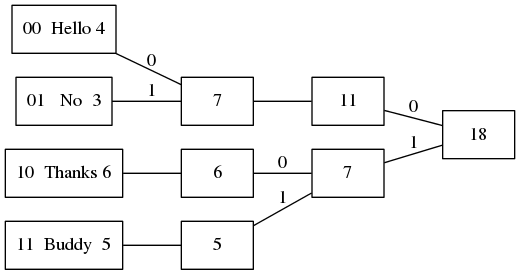
\includegraphics[width=.9\textwidth]{graphs/bht}
\end{center}

From left to right the two nodes with lowest count are
combined into a parent.  Encodings are read off of the splits
 from right to left. 


\end{frame}

\end{document}






























